\documentclass[a4paper]{article}
\usepackage[T1,T2A]{fontenc}
\usepackage[utf8]{inputenc}
\usepackage[english,russian]{babel}
\usepackage{booktabs}
\usepackage{color,colortbl}
%\usepackage{amsmath}
%\usepackage{amsfonts}
%\usepackage{amssymb}
%\usepackage{makeidx}
\usepackage{listings}
\usepackage{graphicx}
\usepackage{rotating}
\definecolor{green}{RGB}{45,140,31}
\definecolor{darkishgreen}{RGB}{39,203,22}
\definecolor{LightCyan}{rgb}{0.88,1,1}
\definecolor{Gray}{gray}{0.9}
\definecolor{lightRed}{RGB}{230,170,150}
\definecolor{modRed}{RGB}{230,82,90}
\definecolor{strongRed}{RGB}{230,6,6}

\lstset{ %
  language=python,                % Язык программирования
  numbers=left,                   % С какой стороны нумеровать
  extendedchars=\true,
  %numberstyle=tinycolor{gray},     % Стиль который будет использоваться для нумерации строк
  %stepnumber=2,                   % Шаг между линиями. Если 1, то будет пронумерована каждая строка
 % numbersep=5pt,
 % backgroundcolor=color{white},      % Цвет подложки. Вы должны добавить пакет color - usepackage{color}
  showspaces=false,
  showstringspaces=false,
  showtabs=false,
  %frame=single,                    % Добавить рамку
  %rulecolor=color{black},
  tabsize=4,                       % Tab - 2 пробела
  breaklines=true,                 % Автоматический перенос строк
  breakatwhitespace=true,          % Переносить строки по словам
  title=lstname,                   % Показать название подгружаемого файла
  keywordstyle=\color{green},          % Стиль ключевых слов
  %commentstyle=color{dkgreen},       % Стиль комментариев
  %stringstyle=color{mauve}          % Стиль литералов
}

\usepackage[english,russian]{babel}

\begin{document}

\newpage
\section{Лабораторная работа №3.\newline Разработка графического приложения с использованием спрайтовой анимации}

Цель работы: Научиться реализовывать спрайтовую анимацию в приложениях

\subsection{Теоретические основы}

\textbf{Спрайт} --- графический объект в компьютерной графике. Чаще всего --- растровое изображение, которое можно отобразить на экране. Изначально под спрайтами понимали небольшие рисунки, которые выводились на экран с применением аппаратного ускорения. На некоторых машинах (MSX 1, NES) программная прорисовка приводила к определённым ограничениям, а аппаратные спрайты этого ограничения не имели. Впоследствии с увеличением мощности центрального процессора от аппаратных спрайтов отказались и понятие «спрайт» распространилось на всех двумерных персонажей. В частности, в видеоиграх Super Mario и Heroes of Might and Magic вся графика спрайтовая, анимированная с помощью перебора изображений из атласа спрайтов. К аппаратно ускоренным спрайтам вернулись в середине 1990-х годов — когда развитие мультимедиа и взрывное повышение разрешения и глубины цвета потребовало специализированного процессора в видеоплате. Именно тогда, как обёртка над аппаратным 2D-ускорителем, вышел DirectDraw. DirectX 8 ввёл общий API для двух- и трёхмерной графики, и в современных спрайтовых играх двухмерные спрайты выводятся точно так же, как и трёхмерные — как текстурированный прямоугольник. Атлас спрайтов (Рис.~\ref{ris:heroes}) является растровым изображением, объединяющим спрайты в набор раскадровок анимаций, или иным комплектом спрайтов. Целесообразность применения заключается в уменьшении количества файлов и применение sprite-batch в процессе рендеринга: видеокарте передаётся одно изображение, набор координат, на которых его необходимо «отрендерить» и «трафаретов», вырезающих из атласа отдельные спрайты. В результате, двухмерная графика «рендерится» значительно быстрее, чем одиночными передачами видеокарте одиночных спрайтов с указанием координат отрисовки. Для дополнительного сжатия и уменьшения количества неиспользуемого пространства, атлас может комбинировать изображения не сеткой, а в максимально плотно сжатом виде, таким образом, что, если описать вокруг каждого спрайта прямоугольник — часть прямоугольников будет пересекаться. Данный формат требует дополнительной информации о вершинах, которыми можно описать каждый спрайт без пересечения с другими, и увеличивает время загрузки приложения, но позволяет сократить память.


\begin{figure}[h]
\center{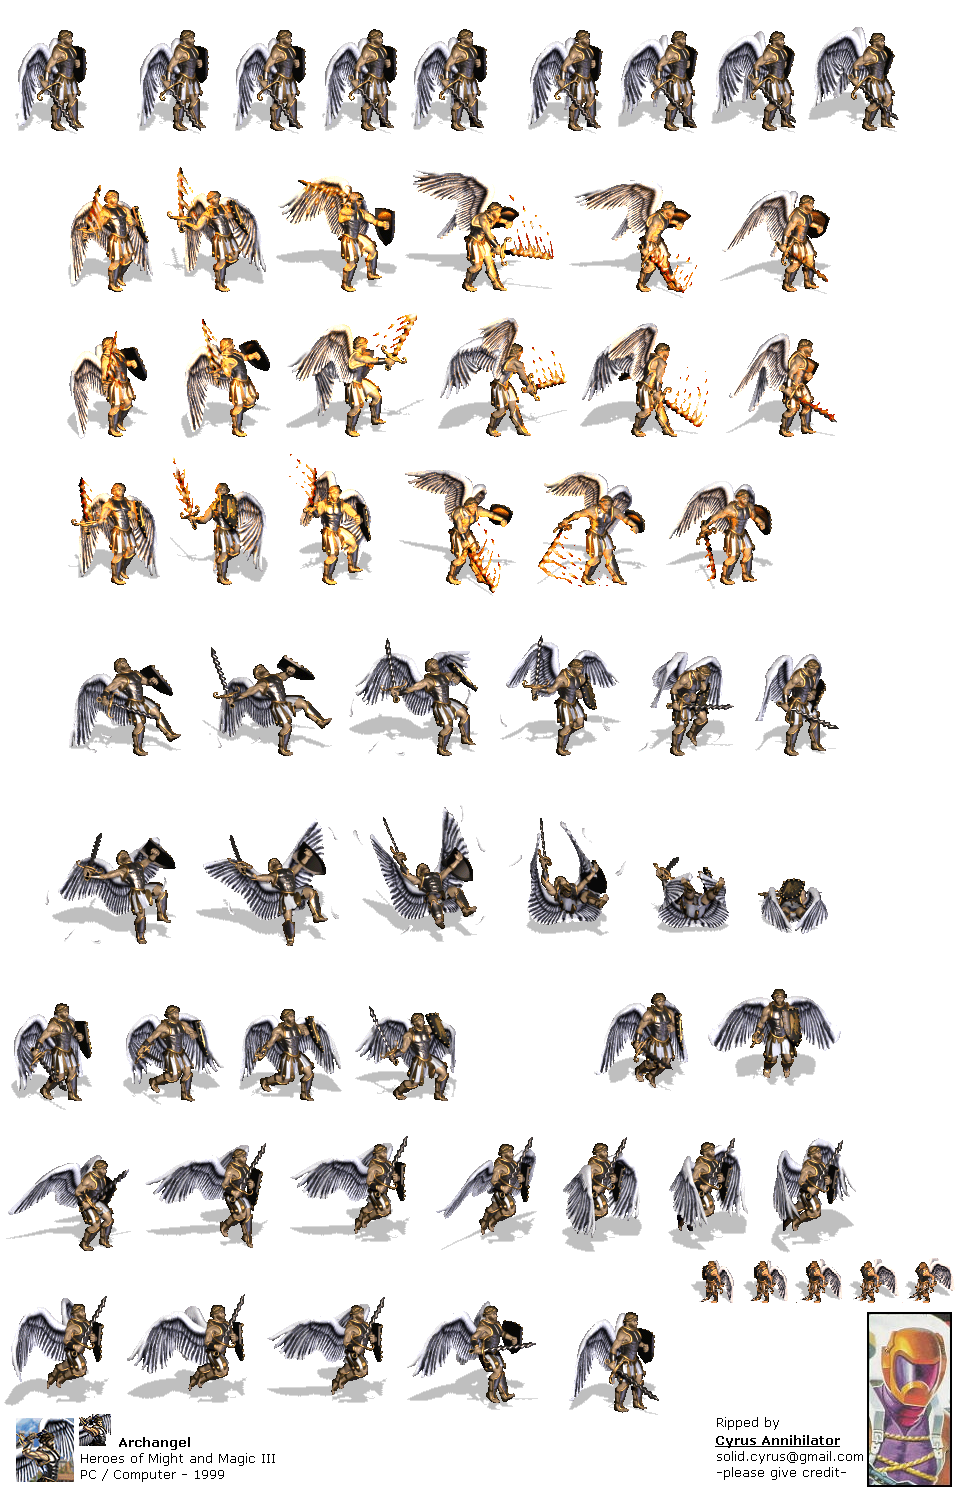
\includegraphics[scale=0.3]{sprite_atlas.png}
  \caption{Атлас спрайтов}\label{ris:heroes}}
\end{figure}

Реализуем в нашем приложении анимацию загрузки с помощью  спрайтовой анимации. В библиотеке tkinter для отображения рисунков отвечает объект canvas который представляет из себя ``холст-объект'' на котором можно размещать различные объекты и фигуры.

Для анимации, вместо нескольких изображений или атласа спрайтов, можно разбить gif файл на набор фреймов (Листинг~\ref{giftoframe})

\newpage
\begin{lstlisting}[label=giftoframe,caption=Выборка данных][h]
frames = []
for i in range(100):
    try:
        frames.append([PhotoImage(file='loading.gif',format = 'gif -index %i' %(i))])
    except:
        break
\end{lstlisting}

Затем создаем функцию анимации в которой покадрово меняем изображение (Листинг~\ref{anim})

\begin{lstlisting}[label=anim, caption=Функция анимации][h]
def anim():
    i = 0

    def next_shot():
        nonlocal i
        canvas.create_image(0, 0, anchor='nw', image=frames[i])
        if i < len(frames) - 1:
            i += 1
            root.after(50, next_shot)
        else:
            canvas.destroy()
            canvas2.destroy()

    return next_shot
\end{lstlisting}

Когда цикл анимации закончится мы просто разрушаем объект. Стоит понимать что ранее разработаная прорамма ``Список дел'' - простая программа и работает достаточно быстро. Что бы анимация была заметна, она будет добваленна при загрузке приложения вне зависимости как быстро загрузилась программа.

\lstinputlisting[caption='Список дел со спрайтовой анимацией', language=Python]{todo_with_sprite.py}

\newpage
\subsection{Задание на лабораторную работу}

Для выполнения работы необходимо:
\begin{enumerate}
  \item Изучить теоретический материал
%  \item Выбрать задание в соответствии с вариатом
  \item Добавить в ранее написаную программу работу со спрайтами
  \item Опубликовать код на github и предоставить ссылку в отчете
  \item Оформить отчет по лабораторной работе
\end{enumerate}

\subsection{Содержание отчета}
\begin{enumerate}
  \item Титульный Лист
  \item Цель работы
  \item Краткие теоретические сведения по теме лабораторной работы
  \item Выполненое задание
  \item Ссылка на github
  \item Краткий вывод о проделанной работе
\end{enumerate}

\begin{thebibliography}{3}
  \bibitem{python}Сузи, Р. А. Язык программирования Python : учебное пособие / Р. А. Сузи. — 3-е изд. — Москва : Интернет-Университет Информационных Технологий (ИНТУИТ), Ай Пи Ар Медиа, 2020. — 350 c. — ISBN 978-5-4497-0705-5. — Текст : электронный // Электронно-библиотечная система IPR BOOKS : [сайт]. — URL: http://www.iprbookshop.ru/97589.html
  \bibitem{tkinter} Документация стандартной библиотеки Python : tkinter — Python interface to Tcl/Tk [cайт]. --- URL: https://docs.python.org/3/library/tkinter.html
\end{thebibliography}


\end{document}
